% !TEX root = morphkasten.tex

\section{Entladen}


%##############
\subsection{Kippen}

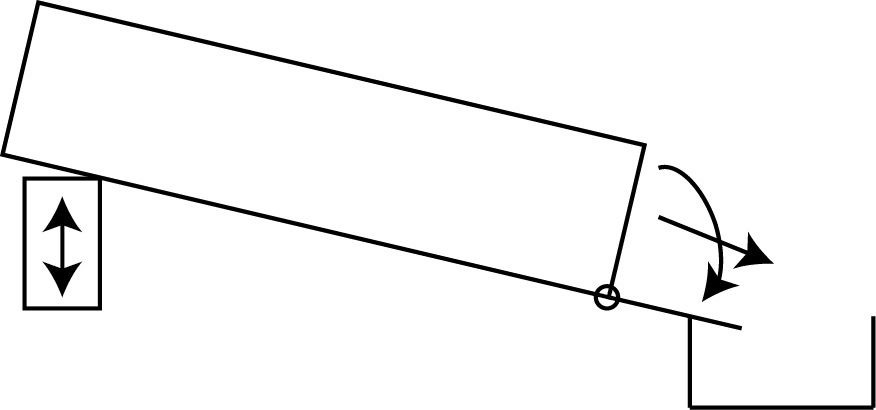
\includegraphics[width=0.5\textwidth]{fig/Entladen_Kippen.png}

\begin{table}[h]
\begin{tabular}{p{0.5\textwidth} | p{0.5\textwidth}}


 \textbf{Vorteile} & \textbf{Nachteile} \\ \hline
	 
\begin{itemize}
\item Kippwinkel kann eingestellt werden
\item Problemloses abladen des Schüttgutes
\end{itemize}

 
 &
 
\begin{itemize}
\item Motor für Kippen notwendig
\item Drehgelenk an Entladebehälter notwendig
\end{itemize}

\end{tabular}
\end{table}

\begin{table}[h]
\begin{tabular}{p{0.5\textwidth}p{0.5\textwidth}}


 \textbf{Risiken} & \\ \hline
	 
\begin{itemize}
\item unpräzises Anfahren des Abladebehälters
\end{itemize}

 
\end{tabular}
\end{table}

\pagebreak


%##############
\subsection{Schrägbehälter}

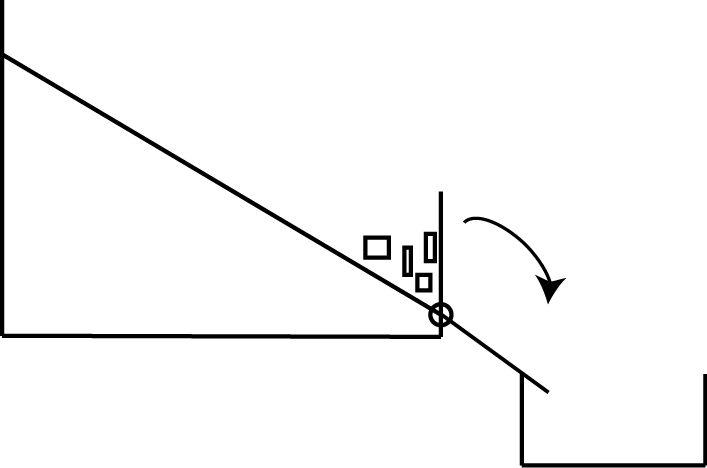
\includegraphics[width=0.5\textwidth]{fig/Entladen_Schraegbehaelter.png}

\begin{table}[h]
\begin{tabular}{p{0.5\textwidth} | p{0.5\textwidth}}


 \textbf{Vorteile} & \textbf{Nachteile} \\ \hline
	 
\begin{itemize}
\item Vorteil 1
\item Vorteil 2
\item Vorteil 3
\item ...
\end{itemize}

 
 &
 
\begin{itemize}
\item Nachteil 1
\item Nachteil 2
\item Nachteil 3
\item ...
\end{itemize}

\end{tabular}
\end{table}

\begin{table}[h]
\begin{tabular}{p{0.5\textwidth}p{0.5\textwidth}}


 \textbf{Risiken} & \\ \hline
	 
\begin{itemize}
\item Risiko 1
\item Risiko 2
\end{itemize}
&
\begin{itemize}
\item Risiko 3
\item ...
\end{itemize}

 
\end{tabular}
\end{table}

\pagebreak